This layer is the heart of the core autonomous functionalities of the Turing Board. We use computer
vision and depth imagery to determine the board's surroundings and calculate the best path to move
forward. The user will have, strapped around their ankle, an anklet-like contraption consisting of a
pattern of ArUco markers for the Follow Along feature (see section 7.7 for more information about the anklet). This layer tracks the movement of the user
through the anklet to determine how to instruct the combination of motors to move so as to follow the
user at an appropriate pace. It is also responsible for detecting possible obstacles when operating on its
own to find the user as part of the Summon feature.

\subsection{Layer Hardware}
The required hardware components include the NVIDIA Jetson TX2 as the main compute module and the Intel RealSense  D432 Depth Camera.

\subsection{Layer Operating System}
The NVIDIA Jetson TX2 is running Ubuntu 18.04. 

\subsection{Layer Software Dependencies}
This layer requires the OpenCV v4.2.2 or higher compiled with cuDNN enabled. A more detailed and exhaustive list can be obtained from. https://github.com/TuringBoard/turing-board-vision/blob/main/
Configuring\%20the\%20NVIDIA\%20Jetson\%20TX2.md.

\subsection{RGB Imagery Subsystem
}
RGB Imagery of the front of the board is used as input in making various position specific calculations pertaining to navigation.

%%%%%%%%%%%%%%%%%%%%%%%%%%%%%%%%%%%%%%%%%%%%%%%%%%%%%%%%%%
%  BE SURE TO UPDATE THE IMAGE CAPTION
\begin{figure}[h!]
	\centering
 	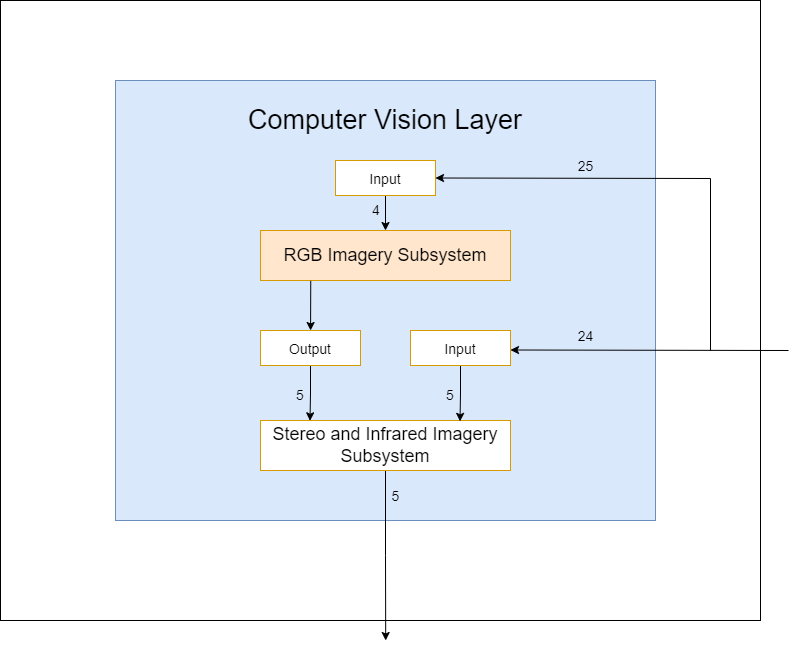
\includegraphics[width=0.60\textwidth]{images/CV_RGB.png} % Image
 \caption{RGB Imagery Subsystem in Computer Vision Layer} % Caption
\end{figure}

\subsubsection{Subsystem Hardware}
The RGB imagery subsystem requires the NVIDIA Jetson TX2 and the Intel RealSense  D432 Depth Camera.

\subsubsection{Subsystem Operating System}
The NVIDIA Jetson TX2 used Ubuntu 18.04 as an operating system.  

\subsubsection{Subsystem Software Dependencies}
The RGB imagery subsystem requires the OpenCV v4.2.2 or higher compiled with cuDNN enabled. A more detailed and exhaustive list can be obtained from. https://github.com/TuringBoard/turing-board-vision/blob/main/Configuring\%20the\%20NVIDIA\%20Jetson\%20TX2.md.

\subsubsection{Subsystem Programming Languages}
The code required for the RGB imagery subsystem is written in Python 3.x.

\subsubsection{Subsystem Data Structures}
The data structure used by the RGB imagery subsystem are:
\begin{itemize}
    \item Arrays
    \item HashMaps
    \item Graphs
    \item Trees
\end{itemize}

\subsubsection{Subsystem Data Processing}
The RGB imagery subsystem processes data using:
\begin{itemize}
    \item SIFT
    \item RANSAC
    \item Canny Edge Detection
\end{itemize}

\pagebreak
% added for figure continuity 

\subsection{Stereo Imagery Subsystem}
Stereo and Infrared Imagery of the front of the board is used as input in making various depth specific calculations pertaining to navigation.

%%%%%%%%%%%%%%%%%%%%%%%%%%%%%%%%%%%%%%%%%%%%%%%%%%%%%%%%%%
%  BE SURE TO UPDATE THE IMAGE CAPTION
\begin{figure}[h!]
	\centering
 	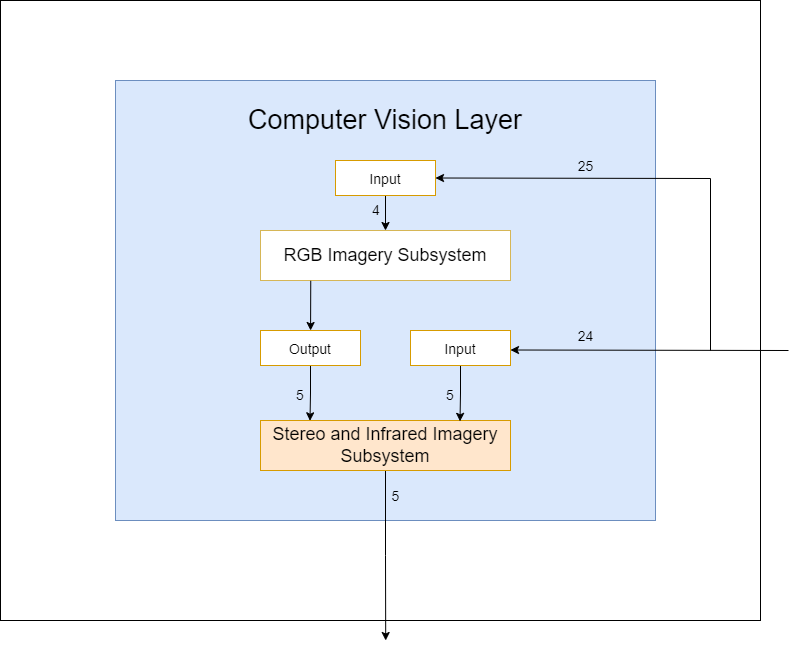
\includegraphics[width=0.60\textwidth]{images/CV_SIR.png} % Image
 \caption{Stereo Imagery Subsystem in Computer Vision Layer} % Caption
\end{figure}


\subsubsection{Subsystem Hardware}
The stereo imagery subsystem requires the Intel RealSense D432 Depth Camera.

\subsubsection{Subsystem Operating System}
The stereo imagery subsystem does not utilize an operating system.

\subsubsection{Subsystem Software Dependencies}
The stereo imagery subsystem has the following software dependencies:
\begin{itemize}
    \item pyrealsense: https://pypi.org/project/pyrealsense
    \item librealsense: https://github.com/IntelRealSense/librealsense 
\end{itemize}

\subsubsection{Subsystem Programming Languages}
The code required for the stereo imagery subsystem is written in Python 3.x.

\subsubsection{Subsystem Data Structures}
The data structure used by the stereo imagery subsystem are:
\begin{itemize}
    \item Arrays
    \item HashMaps
    \item Graphs
    \item Trees
\end{itemize}

\subsubsection{Subsystem Data Processing}
The stereo imagery subsystem processes data using:
\begin{itemize}
    \item SIFT
    \item RANSAC
\end{itemize}
